\chapter{System Design in General}
\label{chap:generalsystemdesign}
In the previous chapter we learned about the different elements that need to be included in a video game, and we will now look into system design in general. When developing a system, there are several aspects to take into consideration. What is the system going to be? What functionality shall the system hold, and what should the system look like? Who are the users, and what are their needs? What software should the system be built upon? There are many questions to be asked and figured out before starting with the development. In this thesis the system is an exergame, the users are elderly people and the exergame will be developed for the Microsoft Kinect technology.

In this chapter we will present theory about some important aspects of system development. We will in Section \ref{sec:fourpillarsofdesign} look into general guidelines for how to design a system. An important part of system design is to set up system requirements. This will be presented in Section \ref{sec:systemreq}. We will also discuss various aspects of usability, which is important to take into account in the process of system development. This will be found in Section \ref{sec:usability}. The aspect of usability is especially important when developing this exergame, due to the users' inexperience with technology.  At the end of this chapter we will present a list of heuristics for games, implemented in a model of "flow". This model will serve as a good way to evaluate video games' usability and for developing games in an early phase.

\section{The Four Pillars of Design}
\label{sec:fourpillarsofdesign}
It is the work of an interactive system designer to combine the sense of what attracts the user with system functionality. To help these designers develop successful systems, a theory called the four pillars of design has been developed. The four pillars of design does not guarantees brilliant systems, but it could be helpful along the way in a development process. The four pillars of design consist of \emph{user interface requirements}, \emph{guidelines documents and processes}, \emph{user-interface software tools} and \emph{expert reviews and usability testing} \cite{mmi}. Each of these pillars will be briefly described next. 

\subsubsection{User Interface Requirements (Ethnographic Observations)}   
As a part of a development process, designers have to specify system requirements. Here, a key to success is to identify and understand the users and their needs, and from that specify user requirements. The way to state these requirements differs from system to system, but what the final result always should include is the same, the system's \emph{context of use}: who should use the system, where should it be used and what should it be used for \cite{mmi}. A good way to understand the users well enough to specify user requirements, is to observe users in action with the system's context and environment. However, the user requirements are only a part of the system's overall requirements. These overall requirements, will, in addition to the user requirements, include specification of software, hardware, response time, etc. All these aspects are important to specify, as it is the overall requirements that form the foundation for the development of the system \cite{mmi} \cite{systemutviklingDel1}. 

\subsubsection{Guidelines Documents and Process (Theories and Models)}
It is important for the interactive system designer to generate a document that obtains a set of guidelines which specifies how the design should be. This could be design guidelines for the whole system, or it can be design guidelines for parts of the system, like functional design, implementation design, and interface design. Companies like e.g. Apple uses guidelines documents to specify design principles developers should follow. This is to create consistency in design across systems and products. Design may differ as different systems have different needs, but there are still some elements that should be considered in the guidelines document. It is important that the guidelines are flexible, so that they can adapt to changes in needs and experiences \cite{mmi}. Examples of what guidelines should describe are:

\begin{itemize}
\renewcommand{\labelitemi}{$\bullet$}
\item Words, icons, and graphics.
\item Screen-layout issues.
\item Input and output devices.
\item Action sequences.
\end{itemize}

\subsubsection{User-Interface Software Tools (Algorithms and Prototypes)}
In the early stages of development, it is difficult for users to picture what the final result will look like. One way to address this problem is to let the users get a realistic impression of the final result, by presenting different types of mock-ups and prototypes of the system \cite{mmi}. What prototypes are, and how and when they should be used, will be presented in Section \ref{sec:prototypes}. When deciding on which development environment to use, there are numbers of good products to choose from. Most of them are easy to use, and offers good features. The important part is for the developers to choose the development environment that is most suitable for the product they are going to make, due to performance, cost, and how easy it is to use and learn \cite{mmi}.
	
\subsubsection{Expert Reviews and Usability Testing (Controlled Experiments)}
To be able to launch a successful system, it is important with testing along the way in the development process. System testing could involve both experts and the intended users \cite{mmi}. 

These four pillars of design form the basis for system development, and, as we see, includes the users along the way in the development process, from system specification to the testing and evaluation phase. This relates to the cycle of user-centered design, which will be described in Section \ref{sec:userinvolvement}.     

\section{System Requirements}
\label{sec:systemreq}
To be able to make a system, designers must start by finding out what the system actually is going to be, what it should do and what functionality that should be included. Finding out and documenting all this is called a requirement analysis. The requirements in this analysis should focus on the role and the purpose of the system, in accordance to the environment the system should be used in. They should include what is essential to the system, and avoid details that are unnecessary. \emph{How} the system is going to be realised, is not common to include in the requirement analysis. From a requirement analysis it is natural to produce what is called a requirement specification \cite{braude2000software}. Requirements specification is defined in \cite{systemutviklingDel1} as \emph{"A specification that sets forth the requirements for a system [...]. Typically included are: functional requirements, performance requirements, interface requirements, design requirements and development standards"}. The different requirements are often separated into two categories, \emph{functional} and \emph{non-functional requirements}. The former specifies \emph{what} functionality the system shall offer, while the latter is about \emph{how} the system shall realise the functionality. 

\subsection{Functional Requirements}
Functional requirements specifies which behaviour, services and functionality the system shall offer its intended users \cite{systemutviklingDel1} \cite{mmi}. Functional requirements are related to the system's context of use, and describe functionality that will be seen by the user. Some examples of functional requirements are listed in \cite{systemutviklingDel1}:
\begin{itemize}
\item \emph{Requirements to ideal functionality and services according to the users' needs and wants.}
\item \emph{Requirements to knowledge about the role of the system, and the environment the system should be used in.}
\end{itemize}     

\subsubsection{Functional Design}
Functional requirements will be used as a primary input to functional design. Functional design should describe the complete functionality of the system that can be seen by the users, and is defined as \emph{"what the system shall do in a way that can be compared to the functional requirements. [...] it provides a basis for selecting the implementation. It is therefore idealised with respect to the concrete system and will hold for a range of technical solutions"}. Functional design is independent from technology and will not say anything about how the system is going to be implemented \cite{systemutviklingDel1}. 

\subsection{Non-Functional Requirements}
Non-functional requirements include performance requirements, interface requirements, reliability and availability requirements, error handling, and constraints. Performance requirements address speed, capacity and memory usage. Reliability and availability requirements specify reliability in quantitative terms, and the amount of time the system should be available to the users. Error handling is about how the system should respond to errors, and interface design says how the system will interact with the users. Constraints restrict how the system should be designed and implemented. This is done by describing accuracy, tool and language to be used, design constraints, which standards that should be used, and the hardware platform the system should be built upon \cite{braude2000software}. To summarise: making non-functional requirements is done to ensure quality of a system, and it describes constraints on hardware, software, and the implementation of the system in general \cite{mmi}. These requirements are hidden from the users' point of view. Examples of non-functional requirements are presented in \cite{systemutviklingDel1} as:
\begin{itemize}
\item \emph{Requirements to physical interfaces.}
\item \emph{Requirements to physical conditions like temperature, humidity, power, consumption etc.}
\item \emph{Requirements to processing capacity: response times, traffic load etc.}
\item \emph{Requirements to exception handling.} \\ \\ 
\end{itemize}   

\subsubsection{Implementation Design}
Non-functional requirements form a basis for implementation design. While functional design is about what the system shall do, implementation design describes how the system should be realised. Implementation design connects the technical solution with the functional design, which makes the "manual" for how the final system will be implemented \cite{systemutviklingDel1}.  

An important part of developing a system is to decide and specify functional and non-functional requirements. It is not always easy to distinguish between the different requirements, in terms of which category they belong under. It is important to notice that categorisation of requirements is not the essential part. What is the main goal is to define and express the requirements as clear, simple and understandable as possible \cite{systemutviklingDel1}. A visual representation of the development process, from requirement specification to implementation, is shown in Figure \ref{fig:requirements}.  

\begin{figure} [H]
\centering
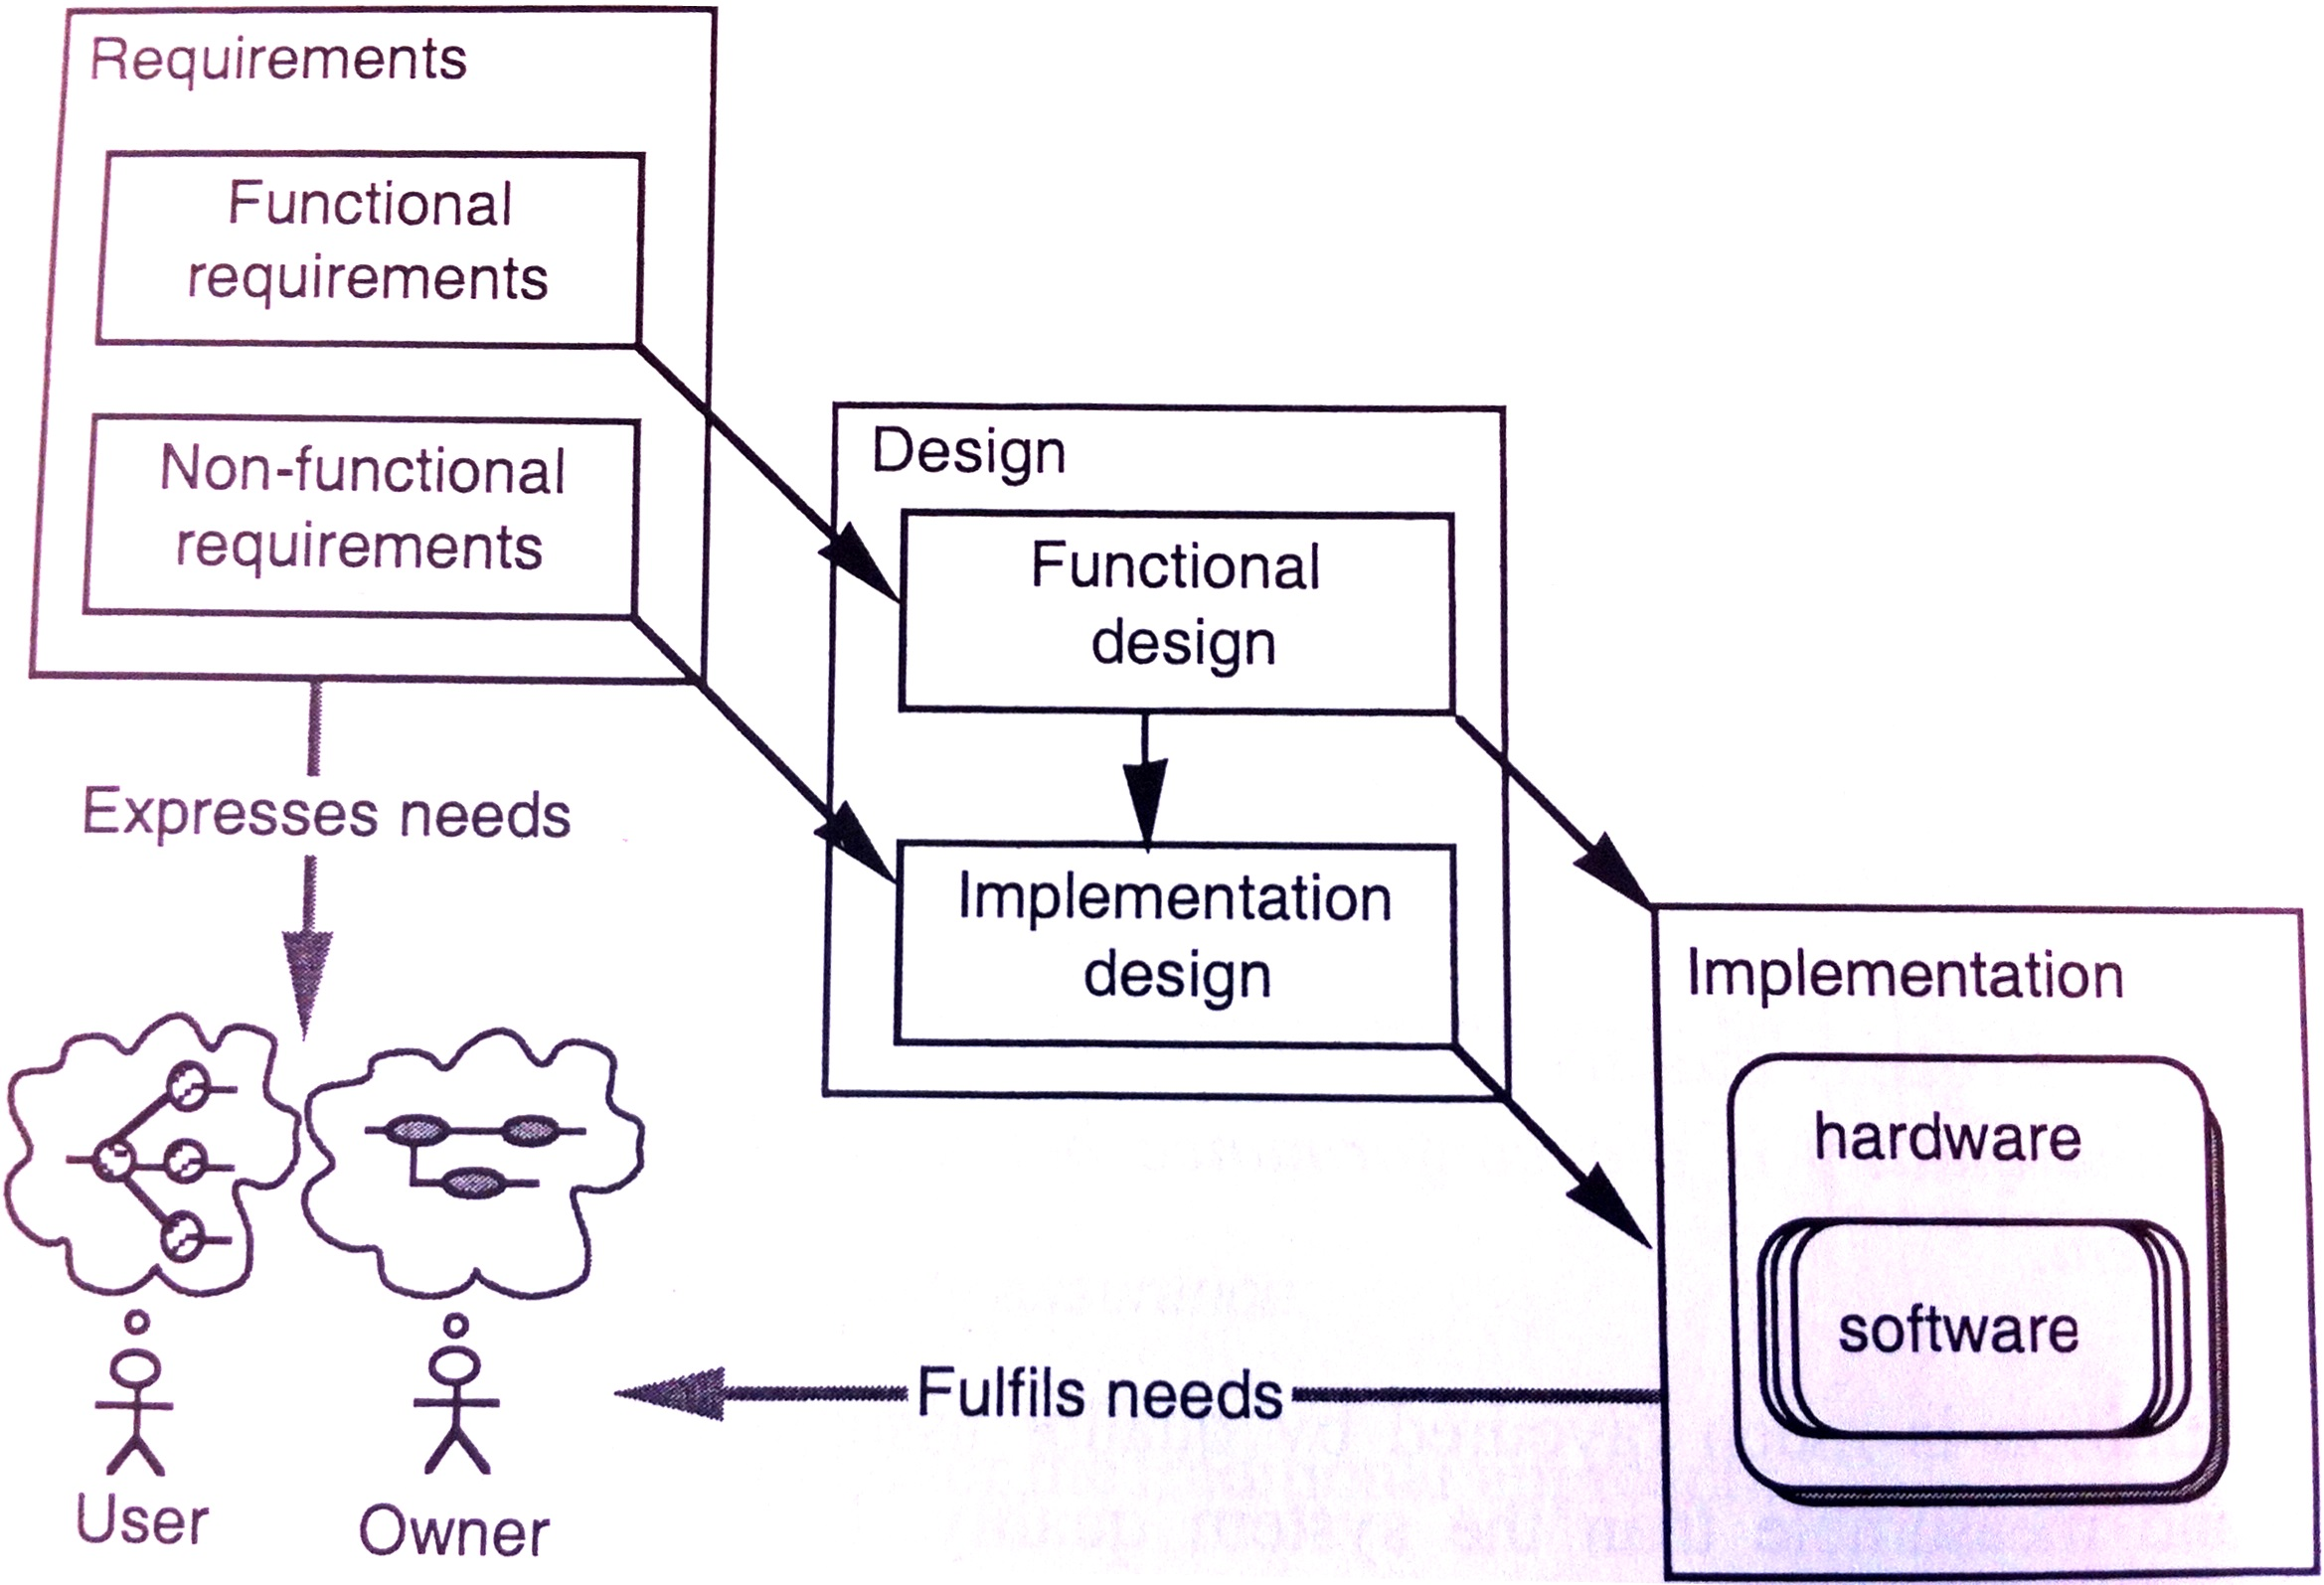
\includegraphics[scale=0.1]{requirements.jpg}
\caption[Main descriptions of system design]{This figure shows the development process from requirement specification to implementation of the system \cite{systemutviklingDel1}.}
\label{fig:requirements}
\end{figure} 

\section{The Importance of Usability}
\label{sec:usability}
When developing a system it is important to keep usability in mind. This term says how easy it is to use, learn and understand a human-made system \cite{mmi}. Usability is often used in association with technology development, in terms of making digital systems understandable and intuitive for the users through user-friendly interfaces. Usability has played a huge part in the evolvement of bringing digital systems into people's homes and everyday life. The first computers and digital systems that were developed consisted of complex and not understandable applications that only professionals with special knowledge could use. There was little focus on simple and accessible systems, and complex interfaces were actually appreciated and gave the system credibility. First, when computers and digital systems were developed with the intention of being used by the normal user, developers had to think about usability. The developers had to put the user in center of the computer system, and not only focus on functionality and system features \cite{mmi}. Users are no longer just "computer professionals", but normal people in all age groups, with different skills and interests, that are both experienced and inexperienced with technology. Putting the users in the center of the system means that the users have to be included in the system's development process. This will be discussed in more detail in Section \ref{sec:userinvolvement}.  

Usability is a wide and quite abstract term, and it is not easy to understand, measure, or practise right. ISO 9241-11 states usability as \emph{"the extent to which a product can be used by specified users to achieve specified goals with effectiveness, efficiency and satisfaction in a specified context of use."} \cite{jokela2003standard}. From this definition we can see that there are three elements that could be helpful in evaluating a system's usability; \emph{effectiveness}, \emph{efficiency} and \emph{satisfaction}. \emph{Effectiveness} measures to which degree systems cover all necessary functionality, and how easy they are to use and understand. \emph{Efficiency} is about how well different tasks are performed. This requires measurement on how much time that is used to accomplish a task. The last element is \emph{satisfaction}, and is about the overall user experience. This could be measures through interviews, studies, questionnaires etc. The degree of satisfaction is important for the system to be accepted \cite{mmi}. 

\subsection{Context of Use}
\label{subsec:contextofuse}
\emph{Context of use} is an important concept within the definition of usability, and is defined in ISO 9241-11 as \emph{"users, tasks and equipment (hardware, software and materials), and the physical and social environment in which a product is used"} \cite{maguire2001context}.  The degree of usability and quality of user experience of a system is dependent on how well it is related to its specified context of use \cite{bevan1995human}. A system will be used by a specific population for specific reasons within a specific environment. It is therefore crucial that the system fits the needs of its intended users, tasks, equipment, and environment. Analysing a system's context of use will help developers to specify who the users are, what are their characteristics, which functionality do they want, and where and in which circumstances do they want to use it. This understanding about a system can be used all through the development process, from system specification to the testing phase \cite{maguire2001context}.

\subsection{Simplicity}
\label{sec:simplicity}

"KISS" and "Less is more" are terms related to usability. "KISS" is an acronym that stands for "Keep it simple, stupid" \cite{kiss2}. This principle was formulated by the American aircraft designer Kelly Johnson in the middle of the 1900s \cite{kiss1}, and it states that simple systems work better than complex ones. KISS is not related to stupidity, but rather to intelligent systems that due to their simplistic design may be perceived as stupid. The KISS principle has been adopted into software engineering, and subjects as design and usability. It states that simplicity should be the main focus in design, and that every element that leads to unnecessary complexity should be avoided \cite{kiss2}. Ludwig Mies van der Rohe was a German architect that used the term "Less is more" to describe his extreme simplistic and minimalistic design style. His use of that term became a guiding principle in modern design, and it has also been adopted as a widely used slogan in association with usability \cite{rohe}. Minimalistic design can be described as \emph{"design at its most basic, stripped of superfluous elements, colors, shapes and textures"} \cite{lessismore}. With minimalistic design, the most important elements are brought into focus. In this way the user will not be distracted from, or miss out on, the content that is important \cite{lessismore}. Also big companies, like Microsoft, focus on simplicity in their design. Microsoft has launched an article called "The Importance of Simplicity" in their developer network. This is about how to design user-friendly systems while still keeping good functionality. In this article, Microsoft presents a topic called "Simple Can Be Powerful", which means that simplistic design not necessarily implies lack of functionality. Simplistic design will provide ease of use for first timers. The idea is to present a design that is intuitive, understandable and easy to learn, with a possibility for the experienced user to choose to add more functionality. A possible solution could be to include customisation so the users can set up their own workspace, and include more features if wanted \cite{msdnsimple}.      

Making good, intuitive, easy to understand systems is essential for a system to be successful, accepted and used. A system can possess the best functionality there is, but if the users do not understand how to use it, the system will fail.      
    
\section{Design Guidelines}
\label{sec:designguide}
In order for a system to become successful it has to be easy to interact with, and it has to offer functionality that is attractive to the user. There have been developed several guidelines to help designers make successful, user-friendly systems. In this section we will present a list of eight principles with focus on interface design, called "The Eight Golden Rules". 

\subsection{The Eight Golden Rules}
\label{subsec:golden}
The "Eight Golden Rules", presented in \cite{mmi}, are a set of guidelines that have been developed over three decades with research and experiences. It does not exist a solution for how to make good and user-friendly interface design, but these "Eight Golden Rules" can serve as a starting point and a helpful design guide if they are used correctly. When using the "Eight Golden Rules", it is important that designers refine and implement the principles into the environment they are working in. 

We will now present the "Eight Golden Rules" \cite{mmi}:

\begin{enumerate}[{e}.1] 
\item \emph{Strive for consistency:} Consistency in interfaces requires identical terminology for actions and layout. This is important for users not to wonder whether words, icons or situations mean the same. 
\item \emph{Cater to universal usability:} Designers have to see the need for making a design that fits the diversity of users. There could be differences in age and technology experience that require transformation of content. Beginners would need guiding and explanations, while experts should have features for shortcuts. This could improve quality of the system experience. 
\item \emph{Offer informative feedback:} The users should always receive feedback on their actions. Appropriate system feedback should be chosen in accordance to the importance of the actions performed. Process bars, sound as a response for clicking a button, or visual presentation for showing objects in actions, are possible ways to give users feedback on actions.  
\item \emph{Design dialogues to yield closure:} It is important to create distinct work steps in dialogues. This means organising similar actions into separate groups with a clear start, middle, and ending. To provide users with a feeling of accomplishment, feedback should be provided when a particular sequence is finished.     
\item \emph{Prevent errors:} The best solution to this problem would be not to experience any errors at all. Designers should prevent users from doing serious errors by e.g. not allowing inappropriate digits in a field or "hiding" buttons that could cause errors. However, when errors do occur users should be provided with informative instructions for how to recover from the problem.   
\item \emph{Permit easy reversal of actions:} Users should always be provided with the possibility to regret a performed action. This will make the system easy and comforting to use, as users know that every action can be undone. 
\item \emph{Support internal locus of control:} Users should feel that they are controlling the interface, and not the other way around. This might be especially important for experienced users. Surprising changes in design and actions, in addition to boring, time-consuming situations, will not be well received. 
\item \emph{Reduce short-term memory load:} Designers should reduce the need for memorising information and how actions should be performed. The focus should be on designing an interface with visible information and intuitive actions.
\end{enumerate}

These presented guidelines are far from being the only guides for how to design a user interface. There have been done a huge amount of research in the area of usability. Jacob Nielsen is one of the researchers \cite{nielsen2005ten}. He is a Ph.D from Denmark, and an expert in human-computer interaction. He has established a movement for how to easy improve user-interfaces, invented several methods for how to achieve good usability, and he has also published a great amount of articles and books with usability as main subject \cite{JNielsen}. As a part of his work Nielsen has created a list of ten usability heuristics, which can be used as general principles when designing a user- interface\cite{nielsen2005ten}. We will now discuss heuristics in more detail.

\section{Heuristics}
\label{sec:heur}
Heuristics are guidelines made to assess how good software design is, and it has become a widely used method for usability evaluation in software development. As learned from this chapter so far, it is important to develop software interfaces that are easy to understand, learn and conduct by the users. Heuristic evaluation methods allow for insight into users' point of view, even before there is an actual system. It is actually best suited in an early phase, before spending a lot of money on expensive prototypes \cite{desurvire}. The heuristics developed by Jacob Nielsen are made for software development in general. These can be found in \cite{nielsen2005ten}. We sought to find heuristics that were more applicable for game development. 

We found that a lot of research has been done on heuristics for games and different sets have been suggested. Some worth mentioning are Desurvire et al. \cite{desurvire}, Malone \cite{malone}, Shelley \cite{shelley}, and Federoff \cite{federoff}. Many of the heuristics overlap, and in some way, they all tell the same. 

Sweetser and Wyeth \cite{sweetser} discovered that many of the heuristics proposed in the literature, did not evaluate the enjoyment in games. They argue that the many valid sets of heuristics presented in the literature should be integrated into a model where also player enjoyment can be assessed. How much someone enjoys something can be described by the concept of flow. The concept of flow was first proposed by  Mihaly Csikszentmihalyi, when he many years ago started to study how people could be so immersed and engaged in something they did not get money for. He wanted to find out why they did these things. He found that the reason was the enjoyment they felt when doing it. He called this state "flow" because \emph{"many of the respondents described the feeling when things were going well as an almost automatic, effortless, yet highly focused state of consciousness"} \cite{flow}.  Sweetser and Wyeth integrated the already existing heuristics into the model of "flow", and called this new model "GameFlow". They argued that the nature of flow fits well as a way to structure the different heuristics found in the literature, into a model of player enjoyment. The "GameFlow" model has eight core elements which are related to Csikszentmihalyi's defined elements. The core elements are: \emph{concentration, challenge, skills, control, clear goals, feedback, immersion} and \emph{social interaction} (see Table \ref{tab:gameFlow}, \ref{tab:gameFlow2}, and \ref{tab:gameFlow3}) \cite{sweetser}. 

These heuristics are proposed generally for games, and every aspect does not have to fit every type of game. However, based on guidelines discussed in Chapters \ref{chap:olderexercise} and \ref{chap:exforseniors} we find most of these aspect relevant also for an exergame for elderly. Therefore, the GameFlow model will be used in our further work, both when evaluating older people's enjoyment of existing commercial games, and when designing the exergame concept. How this model relates to our exergame concept will be presented in Chapter \ref{chap:concept} and discussed in Chapter \ref{chap:discussion}. To come up with a game suitable for elderly people, this user group has to be involved in the development phase. We will now move on to the next chapter, where we will discuss the methods used to involve the user in the development process.

\begin{table} [H]
\centering
\begin{tabular}{|>{\raggedright}p{2,8cm}|p{8,2cm}|}
\hline
\textbf{Element} & \textbf{Criteria} \\ \hline
\textbf{Concentration} Games should & Games should provide a lot of stimuli from different sources. \\ \cline{2-2}
require concentration  & Games must provide stimuli that are worth attending to. \\ \cline{2-2}
and the player should be able & Games should quickly grab the players' attention and maintain their focus throughout the game. \\ \cline{2-2}
to concentrate on the game & Players shouldn't be burdened with tasks that don't feel important. \\ \cline{2-2}
 & Games should have a high workload, while still being appropriate for the players' perceptual, cognitive, and memory limits. \\ \cline{2-2}
& Players should not be distracted from tasks that they want or need to concentrate on.\\ \hline

\textbf{Challenge} Games should  & Challenges in games must match the players' skill levels.\\ \cline{2-2}
be sufficiently challenging and  & Games should provide different levels of challenge for different players. \\ \cline{2-2}
match the player's skill level & The level of challenge should increase as the player progresses through the game and increases their skill level. \\ \cline{2-2}
& Games should provide new challenges at an appropriate pace. \\ \hline
\end{tabular}
\caption[GameFlow criteria for player enjoyment in games, part 1]{GameFlow criteria for player enjoyment in games, part 1 \cite{sweetser}}
\label{tab:gameFlow}
\end{table} 

\begin{table} [H]
\centering
\begin{tabular}{|>{\raggedright}p{2,8cm}|p{8,2cm}|}
\hline
\textbf{Element} & \textbf{Criteria} \\ \hline
\textbf{Player Skills} Games must  & Players should be able to start playing the game without reading the manual. \\ \cline{2-2}
support player skill  & Learning the game should not be boring, but be part of the fun. \\ \cline{2-2}
development and mastery & Games should include online help so players don't need to exit the game. \\ \cline{2-2}
& Players should be taught to play the game through tutorials or initial levels that feel like playing the game. \\ \cline{2-2}
& Games should increase the players' skills at an appropriate pace as the progress through the game. \\ \cline{2-2}
& Players should be rewarded appropriately for their effort and skill development. \\ \cline{2-2}
& Game interfaces and mechanics should be easy to learn and use.\\ \hline

\textbf{Control} Players should feel a sense of & Players should feel a sense of control over their characters or units and their movements and interactions in the game world.\\ \cline{2-2}
 control over their actions in  & Players should feel a sense of control over the game interface and input devices. \\ \cline{2-2}
the game & Players should feel a sense of control over the game shell (starting, stopping, saving etc.). \\ \cline{2-2}
& Players should not be able to make errors that are detrimental to the game and should be supported in recovering from errors. \\ \cline{2-2}
& Players should feel a sense of control and impact onto the game world (like their actions matter and they are shaping the game world). \\ \cline{2-2}
& Players should feel a sense of control over the actions that they take and the strategies that they use and that they are free to play the game the way that they want (not simply discovering actions and strategies planned by the game developers).\\ \hline
\end{tabular}
\caption[GameFlow criteria for player enjoyment in games, part 2]{GameFlow criteria for player enjoyment in games, part 2 \cite{sweetser}}
\label{tab:gameFlow2}
\end{table} 

\begin{table} [H]
\centering
\begin{tabular}{|>{\raggedright}p{2,8cm}|p{8,2cm}|}
\hline
\textbf{Element} & \textbf{Criteria} \\ \hline

\textbf{Clear Goals} Games should  & Overriding goals should be clear and presented early. \\ \cline{2-2}
provide the player with clear goals at appropriate times & Intermediate goals should be clear and presented at appropriate times.\\ \hline

\textbf{Feedback} Players must & Players should receive feedback on progress toward their goals.\\ \cline{2-2}
receive appropriate & Players should receive immediate feedback on their actions. \\ \cline{2-2}
feedback at appropriate times& Players should always know their status or score.\\ \hline

\textbf{Immersion} Players should & Players should become less aware of their surroundings. \\ \cline{2-2}
experience deep but effortless  & Players should become less self-aware and less worried about everyday life. \\ \cline{2-2}
involvement in the game & Players should experience an altered sense of time. \\ \cline{2-2}
& Players should feel emotionally involved in the game. \\ \cline{2-2}
& Players should feel viscerally involved in the game.\\ \hline

\textbf{Social Interaction}  & Games should support competition and cooperation between players.\\ \cline{2-2}
Games should support and  & Games should support social interaction between players (chat, etc.). \\ \cline{2-2}
create opportunities for social interaction & Games should support social communities inside and outside the game.\\ \hline
\end{tabular}
\caption[GameFlow criteria for player enjoyment in games, part 1]{GameFlow criteria for player enjoyment in games, part 3 \cite{sweetser}}
\label{tab:gameFlow3}
\end{table} 


